\documentclass[11pt, oneside]{article}
\usepackage[left=2.5cm,right=2.5cm,top=3cm,bottom=3cm]{geometry}
\usepackage[utf8]{inputenc} 
\usepackage[spanish]{babel}
\geometry{letterpaper}                
\usepackage{graphicx}				
\usepackage{amssymb}
\usepackage{amsmath}
\usepackage{enumerate}
\usepackage{xcolor}
\usepackage{listings}
\usepackage{float}

\lstset{basicstyle=\ttfamily,
  showstringspaces=false,
  breaklines=true,
  commentstyle=\color{red},
  keywordstyle=\color{blue},
  aboveskip=3mm,
  belowskip=3mm,
  frame=tb
}

\title{Git y Github}
\date{}

\begin{document}
\maketitle

\section{Introducción}
Git es un software de control de versiones ó CVS por sus siglas en Ingles. Este tipo de software están diseñados para porder llevar un contro de los cambios en un proyecto en el que esté involucrado el desarrollo de algun tipo de software.

Un ejemplo en el que git es usado bastante es cuando tenemos varias versiones de un proyecto:
\begin{itemize}
  \item tesis.docx
  \item tesis-terminada.docx
  \item tesis-terminada-final.docx
  \item tesis-terminada-fianl-definitiva.docx
\end{itemize}
En lugar de tener tantos archivos diferentes para llevar un control de los cambios, con git tendriamos un solo archivo y este mismo se encargaria de guardar registros de los cambios que se hagan en el proyecto. Aunque estos ejemplos son con archivos de word, git funciona mejor con archivos de texto por ejemplo; .txt, .csv, .c, .java, .tex, etc. Para git es mas dificil especificar los cambios para archivos empaquetados o binarios como .exe, .docx, .pptx, .jpeg, etc.

Otra gran ventaja de git es que permite a muchas personas colaborar en un solo proyecto, de esta forma se puede agilizar el proceso de desarrollo. Para colaborar se pueden utilizar herramientas que implementan el sistema de git como GitHub, GitLab, Bitbucket, etc.

\section{Instalar Git}
Para poder empezar a usar git tenemos que instalarlo, algunos sistemas como Mac o Linux lo podrían tener ya instalado, Windows no trae git instalado así que siempre es necesario instalarlo. Para revisar si ya estan instalados en estos sistemas es necesario abrir el terminal. En linux el terminal se abre presionando las teclas ctrl+alt+t y en Mac se puede abrir el terminal presionando las teclas cmd+espacio y luego ecribiendo la palabra terminal. Una vez abierto el terminal tenemos que escribir el commando:
\begin{lstlisting}[language=bash,caption={Comando para revisar versión de Git}]
git --version
\end{lstlisting}
Si lo tenemos instalado deberiamos ver una linea parecida a la siguiente:
\begin{lstlisting}[language=bash,caption={Versión de Git}]
git version 2.24.3 
\end{lstlisting}
Si no lo tenemos instalado veremos algo parecido a esto:
\begin{lstlisting}[language=bash,caption={Git no instalado}]
Unknown command: git
\end{lstlisting}

En caso que git no este instalado tendremos que ir al sito web \url{https://git-scm.com/downloads} y darle click al botón de descargar. En la figura \ref{fig:git-web} se muestra la pagina donde descargar git.
\begin{figure}[H]
  \centering
  \caption{Sitio web de git}
  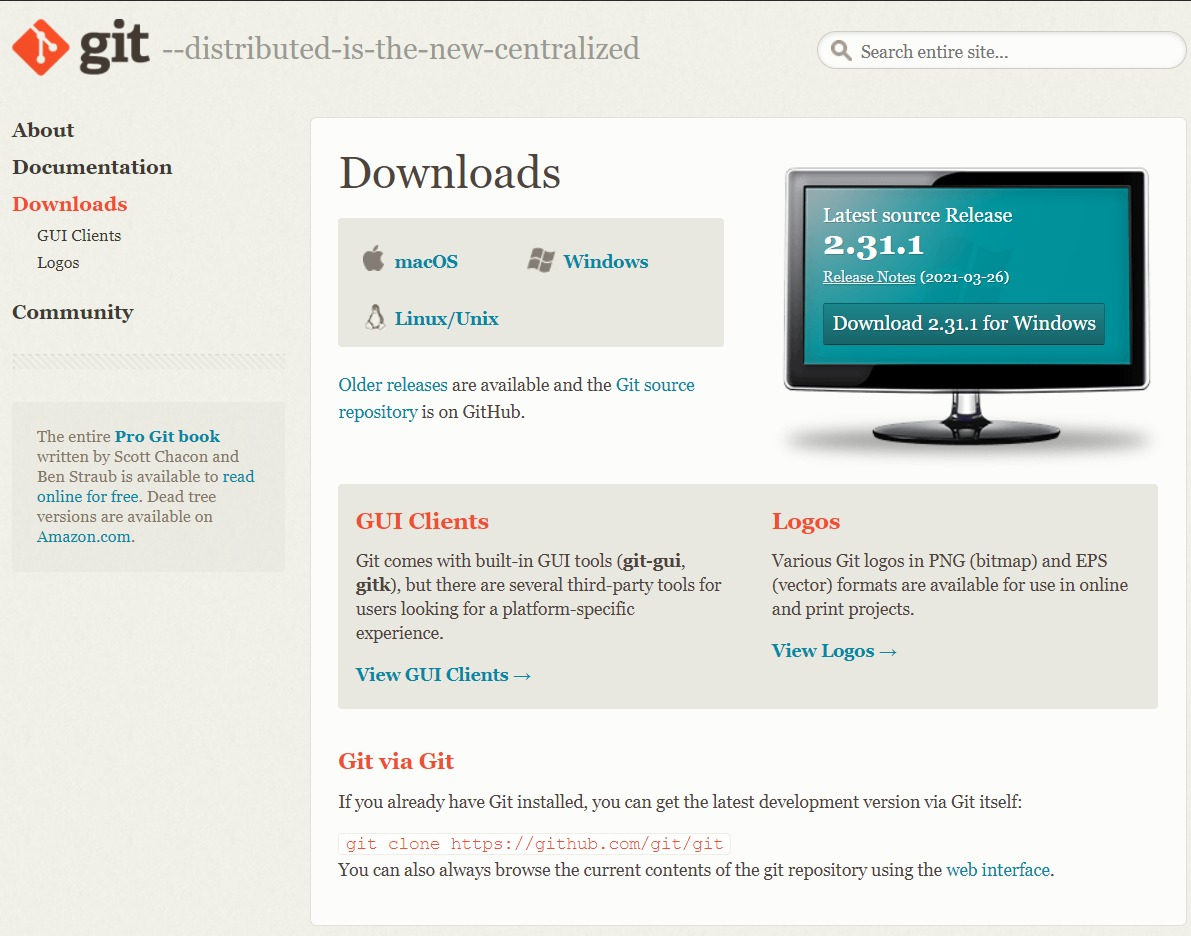
\includegraphics[width=0.70\textwidth]{./img/ind-from-web.jpeg}
  \label{fig:git-web}
\end{figure}

\subsection{Windows}
Una vez descargado el git hay que ejecutar el programa. Aparecera la siguiente ventana y hay que darle click en el botón Ejecutar:
\begin{figure}[H]
  \centering
  \caption{ejecutar programa git}
  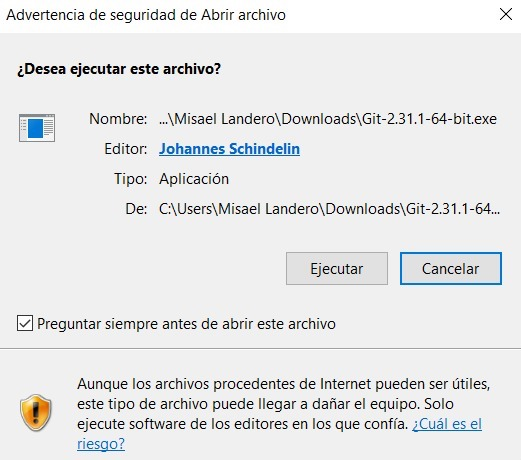
\includegraphics[width=0.50\textwidth]{./img/win/ins-win-1.jpeg}
  \label{fig:git-ins-1}
\end{figure}

Luego se arbrira la ventana de instalación, en la cual le daremos siguiente a la mayoría de las opciones.

\begin{figure}[H]
  \centering
  \caption{ejecutar programa git}
  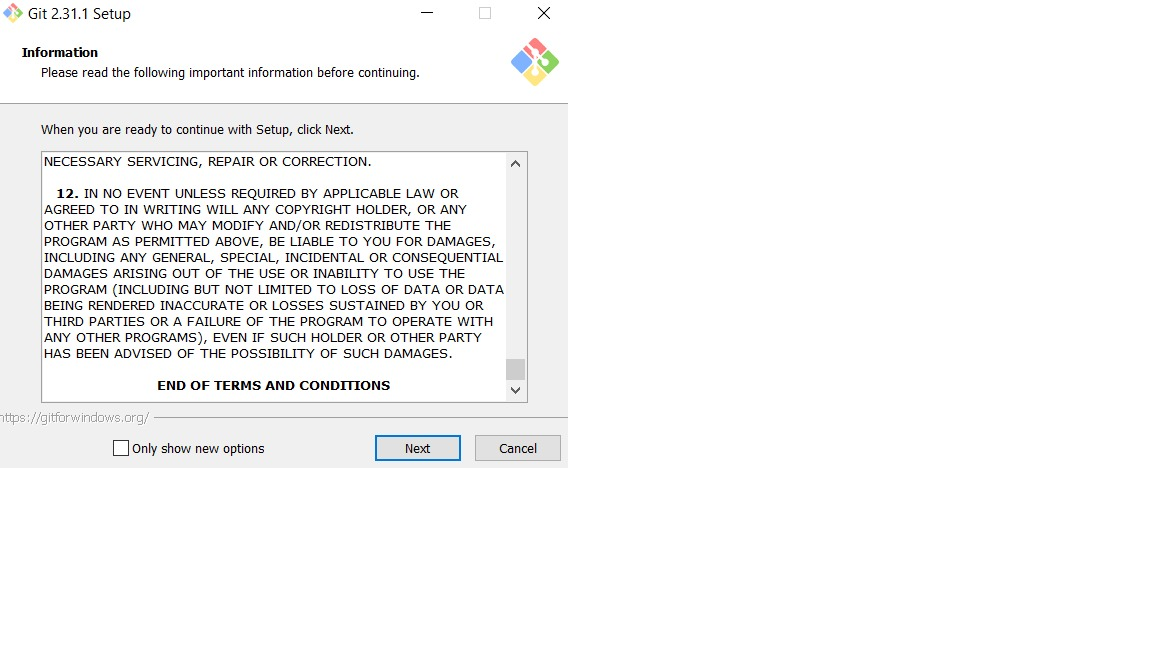
\includegraphics[width=0.50\textwidth]{./img/win/ins-win-2.jpeg}
  \label{fig:git-ins-2}
\end{figure}

Luego de darle click a siguiente una cuantas veces llegaremos a una opción par definir el nombre por defecto de la rama principal, este lo cambiaremos a main en lugar de master ya que GitHub cambió su configuración para que la rama principal se llame main. De esta forma nos ahorraremos cambiarle el nombre a la rama maualmente.

\begin{figure}[H]
  \centering
  \caption{ejecutar programa git}
  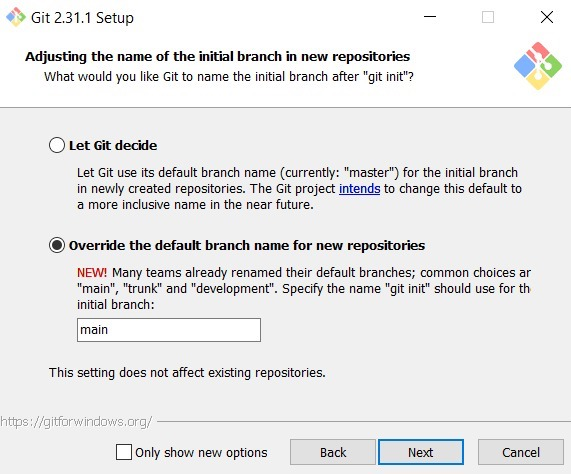
\includegraphics[width=0.50\textwidth]{./img/win/ins-win-3.jpeg}
  \label{fig:git-ins-3}
\end{figure}

La siguiente opción que tendremos que modificar es desde donde podemos ejecutar git, eligiremos la opción de ejecutarlo desde la linea de comando y desde software de terceros (esto nos facilitará usarlo).

\begin{figure}[H]
  \centering
  \caption{ejecutar programa git}
  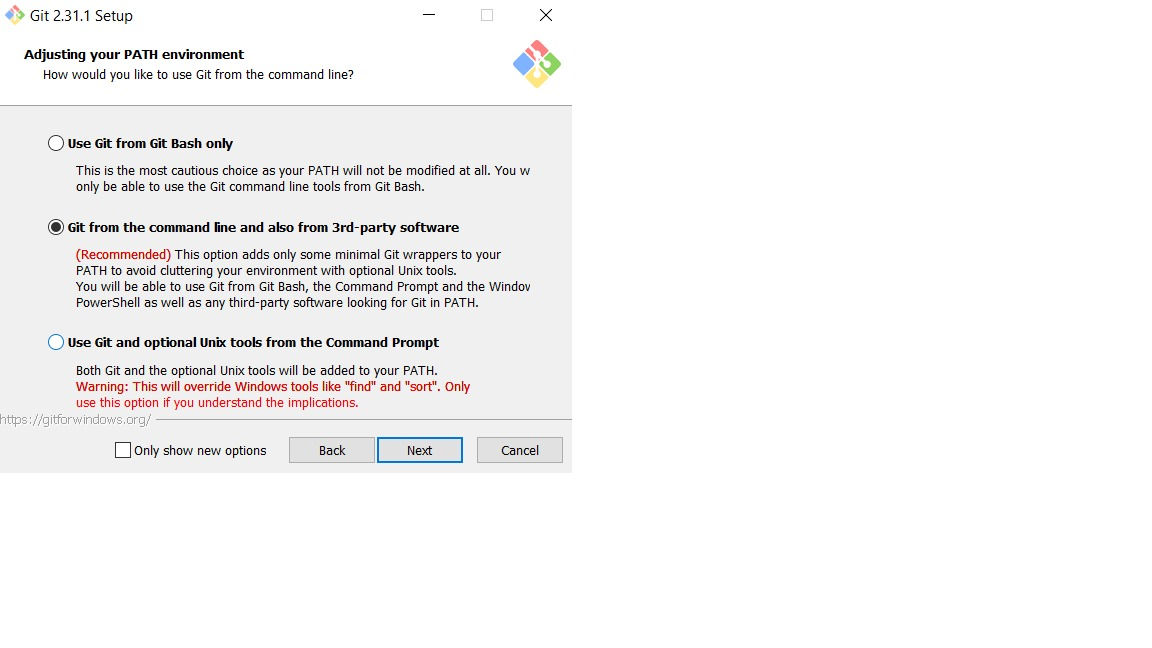
\includegraphics[width=0.50\textwidth]{./img/win/ins-win-4.jpeg}
  \label{fig:git-ins-4}
\end{figure}

La última opción que tenemos que agregar es el de usar pseudo consolas, esto ayuda a poder ejecutar comandos de python o node desde la consoloa de git.

\begin{figure}[H]
  \centering
  \caption{ejecutar programa git}
  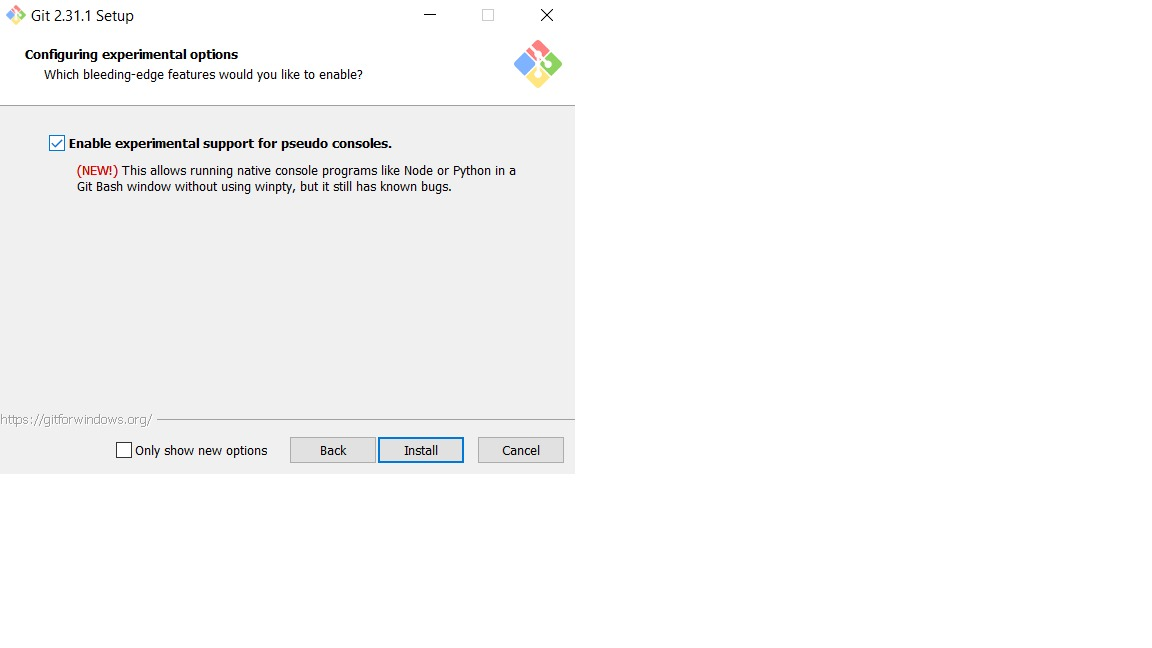
\includegraphics[width=0.50\textwidth]{./img/win/ins-win-5.jpeg}
  \label{fig:git-ins-5}
\end{figure}

Despues de seleccionar la opción anterior le damos click en el botón Instalar y con esto ya tendremos git instalado.

\subsection{Mac}
La instalación de git en mac es mucho mas sencilla, pero antes de poder instalarlo tendremos que instalar un manejador de paquetes. El manejador que paquetes que instalaremos se llama HomeBrew, esta dispobible en el siguiente enlace: \url{https://brew.sh/}.

Para instalar HomeBrew tendremos que abrir el terminal de Mac y escribir el siguiente comando:

\begin{lstlisting}[language=bash,caption={Comando para instalar HomeBrew}]
/bin/bash -c "$(curl -fsSL https://raw.githubusercontent.com/Homebrew/install/HEAD/install.sh)"
\end{lstlisting}

Una vez instalado HomeBrew, instalar git es sencillo. Siempre en el terminal escribiremos el siguiente comando:

\begin{lstlisting}[language=bash,caption={Comando para instalar git en Mac}]
brew install git
\end{lstlisting}

\subsection{Linux}
Por último, instalar git en Linux es mas facil que en los sistemas operativos anteriores. Primero abriremos el termial y luego dependiendo de la distribución de Linux que usemos escribiremos el siguiente comando:

\subsubsection{Ubuntu/Debian}
\begin{lstlisting}[language=bash,caption={Comando para instalar git en Ubuntu}]
apt-get install git
\end{lstlisting}

\subsubsection{Fedora}
\begin{lstlisting}[language=bash,caption={Comando para instalar git hasta Fedora21}]
yum install git
\end{lstlisting}

\begin{lstlisting}[language=bash,caption={Comando para instalar git en Fedora22 y superiores}]
dnf install git
\end{lstlisting}

Para otras distribuciones de linux revisar el siguiente enlace: \url{https://git-scm.com/download/linux}

\section{GitHub}
Github es una plataforma que implemeta Git y hace mas facil poder colaborar con varias personas en proyectos de codigo a traves de la web. GitHub es relativamente sencillo de usar, pero tiene funcionalidades bien robustas para programadores experimentados. 

\subsection{Registrarse en GitHub}
Para empezar a usar GitHub primero hay que crear un perfil en, para esto hay que ir a la dirección web \url{https://github.com/} y hacer click en el botón de la esquina superios izquierda "Sign Up".

\begin{figure}[H]
  \centering
  \caption{Página web de GitHub}
  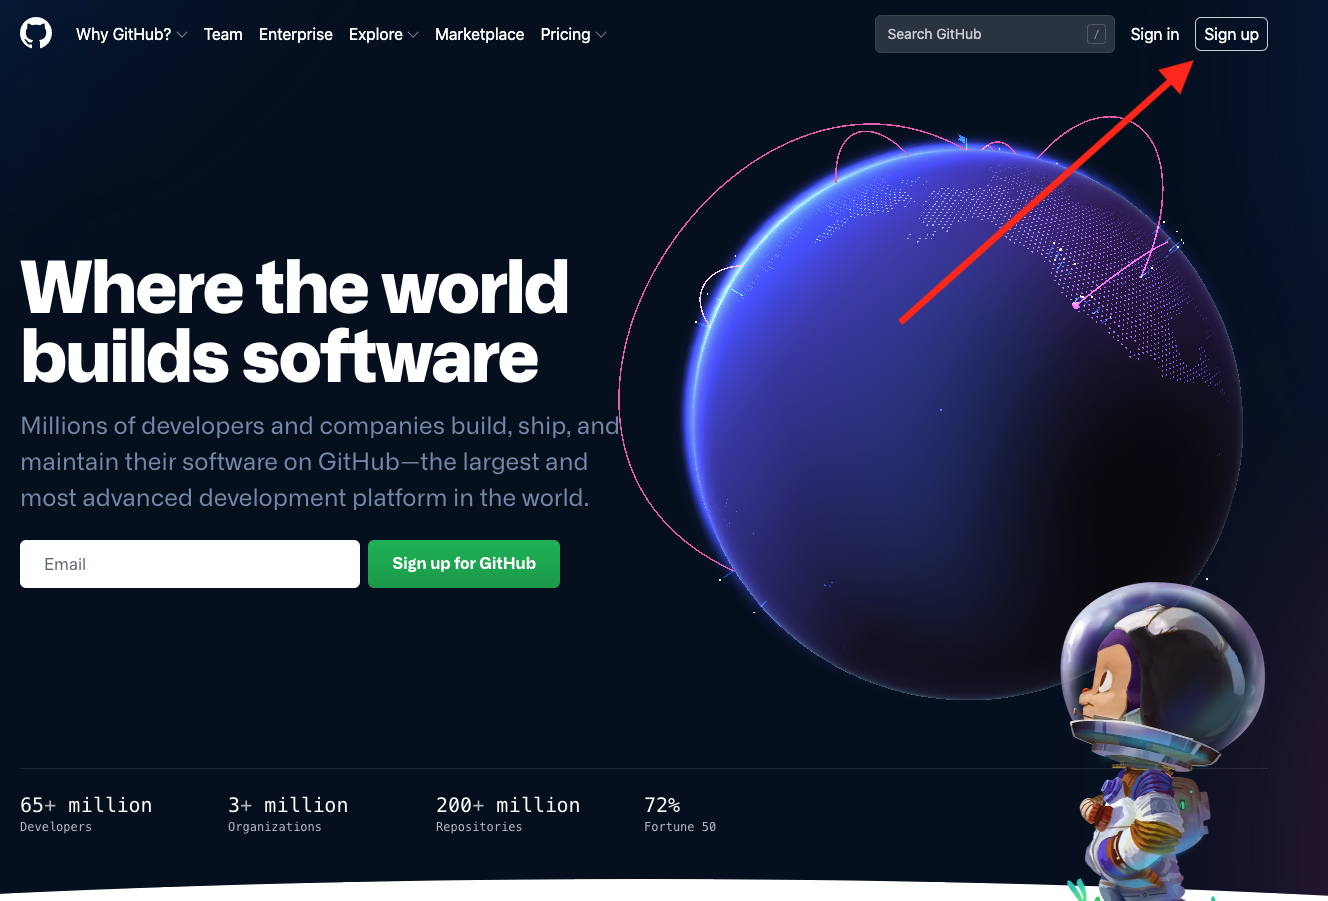
\includegraphics[width=0.90\textwidth]{./img/github-signup-1.png}
  \label{fig:github-signup-1}
\end{figure}

Una vez hayamos dado click en el botón SignUp entratemos a una página donde tendremos que poner nuestros datos para crear la cuenta.

\begin{figure}[H]
  \centering
  \caption{Registrarse en GitHub}
  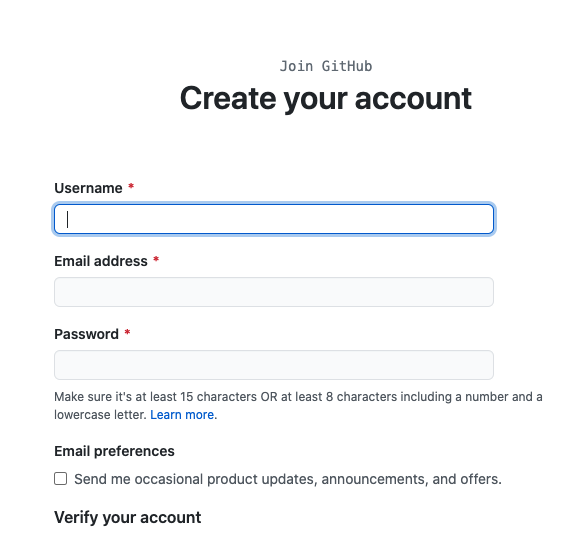
\includegraphics[width=0.50\textwidth]{./img/github-signup-2.png}
  \label{fig:github-signup-2}
\end{figure}

\section{Integración con VSCode}

\section{Integración con VSCode}

\end{document}
